\subsection{Histogram computation}\label{sec:histogram}

\pavol{motivate query; expand with examples}
\duong{what does this mean?}

The computation of a histogram is one of the most common tasks in data analysis. A histogram
succinctly summarizes the distribution of sample values, and thus is useful as a cursory ``look''
into the data, and in guiding further analysis. For example, it can be used to guide the selection
of colors and opacities in transfer functions.

There are several metrics proposed in the literature to measure the distance between two
distributions. We have experimented with the most common ones, namely Kolmogorov-Smirnov [CITE],
Kullback-Leibler [CITE], Hellinger [CITE], Total variation [CITE], Chi-square [CITE], Bhattacharyya
[CITE], Earth Mover's Distance~\cite{emd1998}, $L_1$ norm, and
Intersection~\cite{histogram_intersection1991}. We have found that the relative ordering of streams'
performance do not vary across the distance metrics. Also, it is interesting to note that among the
$s_{opt}$'s streams, the one using the Earth Mover's Distance has the least RMSE. However, we choose
Intersection as the metric of choice, because it is fast to compute, and is the least sensitive to
slight changes in precision. The intersection distance between two histograms $H_1$ and $H_2$ is
defined as $e(H_1,H_2)=\sum_{i}{\min{(H_1(i),H_2(i))}}$ (the sum is over all bins $i$). We normalize
$e$ by dividing it by the total number of samples in the data. Our error metric takes into account
not only the shapes but also the value ranges of histograms. Therefore, when computing the histogram
of a reconstructed function, we clamp its range of values to that of the original function's, so
that corresponding histogram bins, i.e., $H_1(i)$ and $H_2(i)$, share the same range.

As before, for each data set, we use Algorithm\autoref{alg:greedy} to compute an $s_{hist-opt}$
stream, optimized for histogram error, and an $s_{hist-sig}$ from its signature.
\autoref{fig:histogram-stream-comparison} plots the error curves for all relevant streams using the
error metric just defined. We use 64 for the number of bins, but note that there exists no
meaningful differences across a wide range of number of bins (from 64 to 512) in our experiments. In
all cases, the group consisting of $s_{bit}$, $s_{lvl}$, and $s_{mag}$ underperforms the other group
by a large margin.

Among the former group, $s_{lvl}$ generally outperforms $s_{bit}$ at low bit rates, although there
are several crossover points between the two curves. These crossover points are explained in
\autoref{fig:histogram-explain}. When leading zero packets are present, $s_{lvl}$ absolutely
outperforms $s_{bit}$, because increasing resolution does not help producing an accurate histogram
as much as increasing precision. The histogram is oblivious to spatial locations of samples (which
requires resolution to resolve), but it is sensitive to sample values (which requires precision).
However, when leading zero packets are removed, as is the case when using compression, $s_{bit}$
benefits significantly more than $s_{lvl}$ does (for the same reason explained in
\autoref{sec:rmse-optimized}), resulting in the observed crossovers. Finally, $s_{mag}$ performs
poorly, because it ignores regions of smooth variations, which nevertheless counts towards the
distribution.

In the other group, $s_{wav}$'s and $s_{hist-sig}$'s (and even $s_{hist-opt}$'s) performances
differ by negligible amount. This observation is confirmed in \autoref{fig:histograms-boiler}, where
we plot various histograms, reconstructed at 0.08 bps, for the \emph{boiler} data set. The histograms
produced by $s_{wav}$ and $s_{hist-sig}$ have approximately the same shape, and are the closest to
the reference histogram. The next best histogram is produced by $s_{lvl}$, followed by the one
produced by $s_{bit}$, and finally $s_{mag}$. These results suggests that histogram computation is
among analysis tasks that benefit significantly from a bit ordering that combines both resolution
and precision, not one that adheres to either exclusively.

\begin{figure}[t]
	\centering
	\subcaptionbox{\emph{boiler}}
	{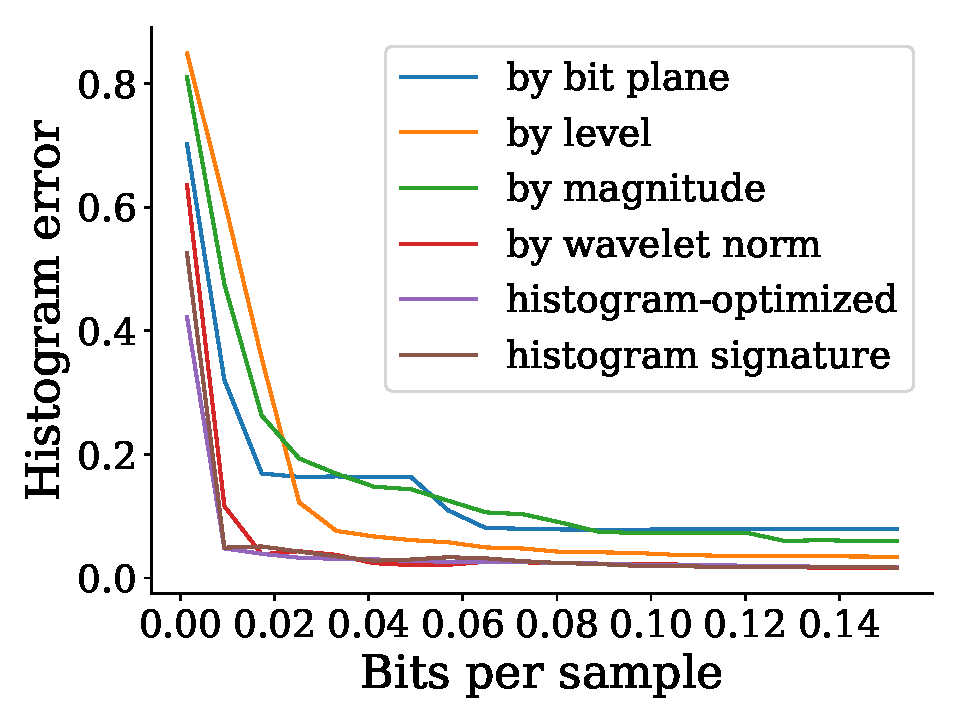
\includegraphics[width=0.48\linewidth]{histogram/histogram-optimized-boiler}}
	\subcaptionbox{\emph{diffusivity}}
	{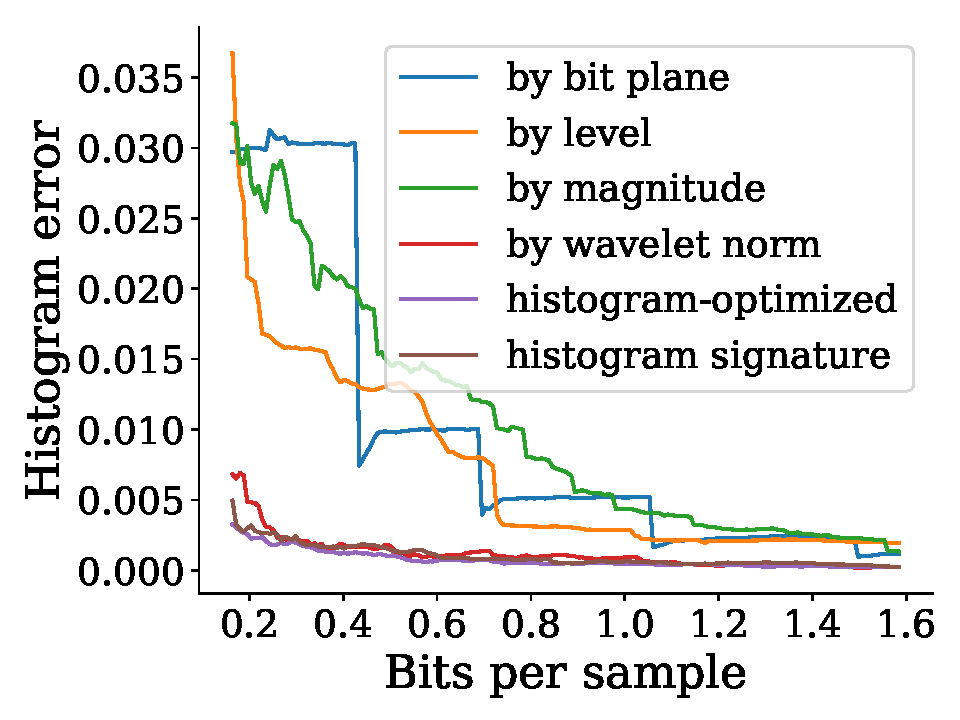
\includegraphics[width=0.48\linewidth]{histogram/histogram-optimized-diffusivity}}
	\subcaptionbox{\emph{plasma}}
	{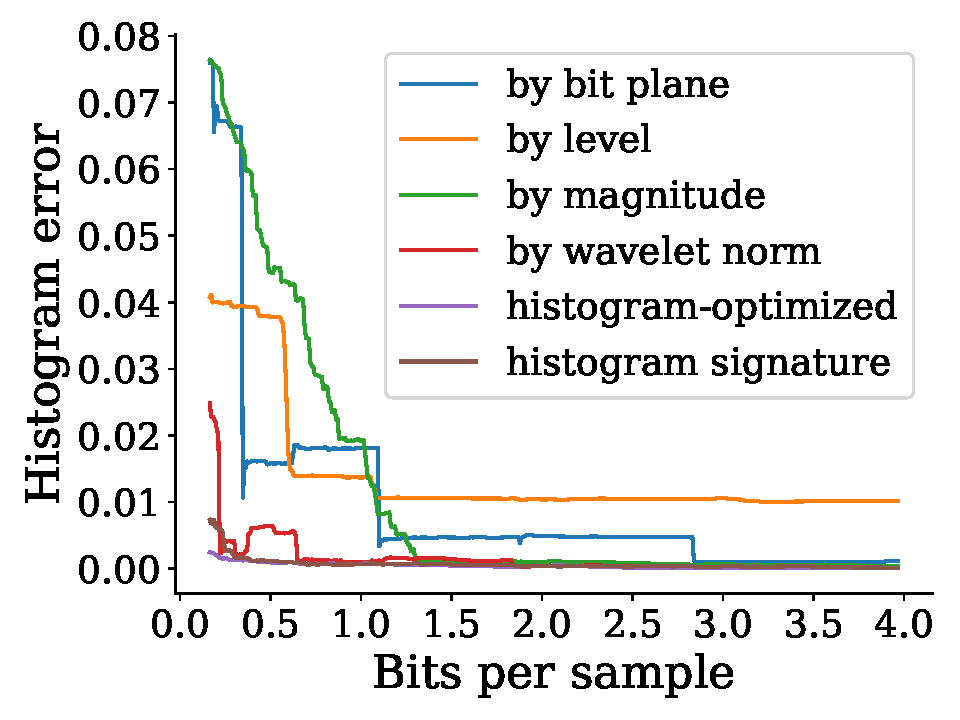
\includegraphics[width=0.48\linewidth]{histogram/histogram-optimized-plasma}}
	\subcaptionbox{\emph{turbulence}}
	{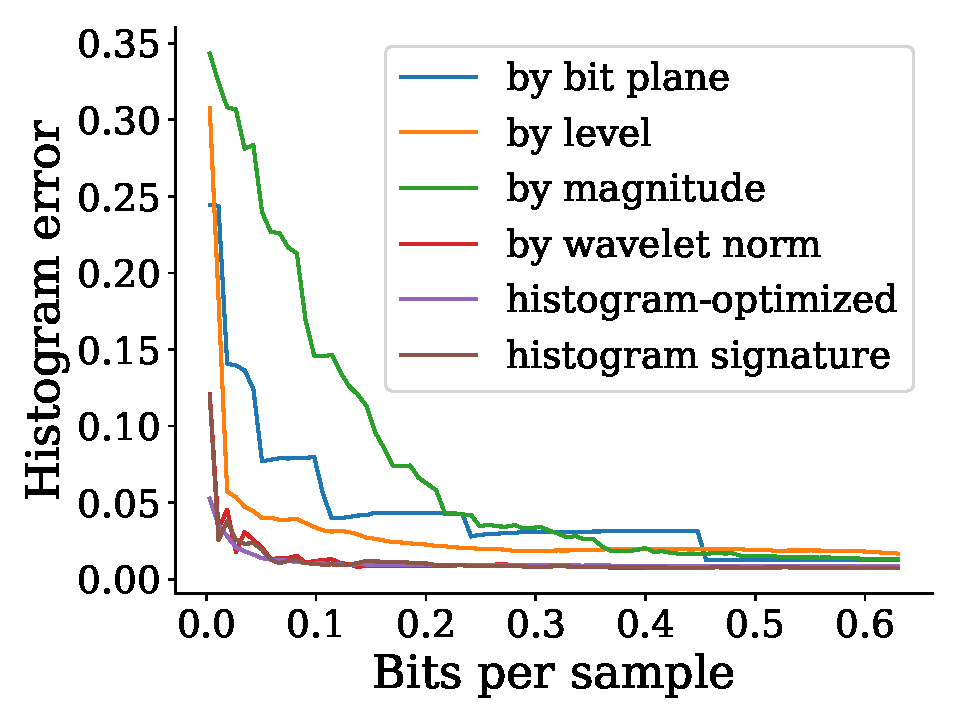
\includegraphics[width=0.48\linewidth]{histogram/histogram-optimized-turbulence}}
	\caption{Comparison of histogram errors among streams. Plots are truncated to highlight
	differences without hiding important trends. In general, $s_{hist-opt}\approx s_{hist-sig}\approx
	s_{wav} > s_{lvl} > s_{bit} > s_{mag}$. Crossover points between $s_{bit}$ and $s_{lvl}$ are
	explained in \autoref{fig:histogram-explain}}.
	\label{fig:histogram-stream-comparison}
\end{figure}

\begin{figure}[t]
	\centering
	\subcaptionbox{with leading zero packets}
	{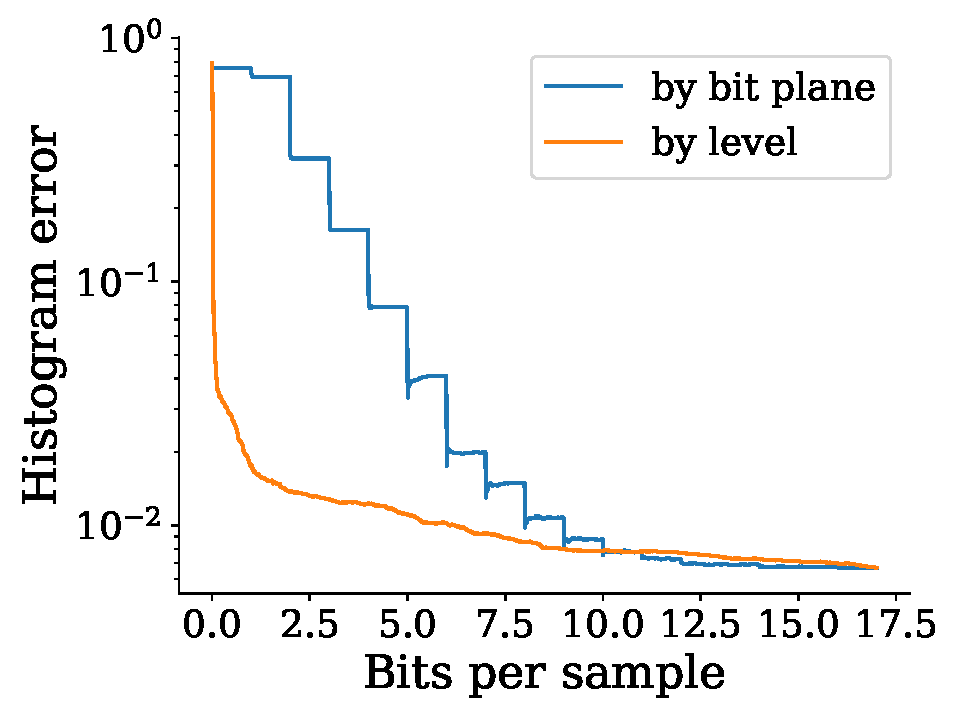
\includegraphics[width=0.48\linewidth]{histogram/histogram-explain-boiler-wlz}}
	\subcaptionbox{without leading zero packets}
	{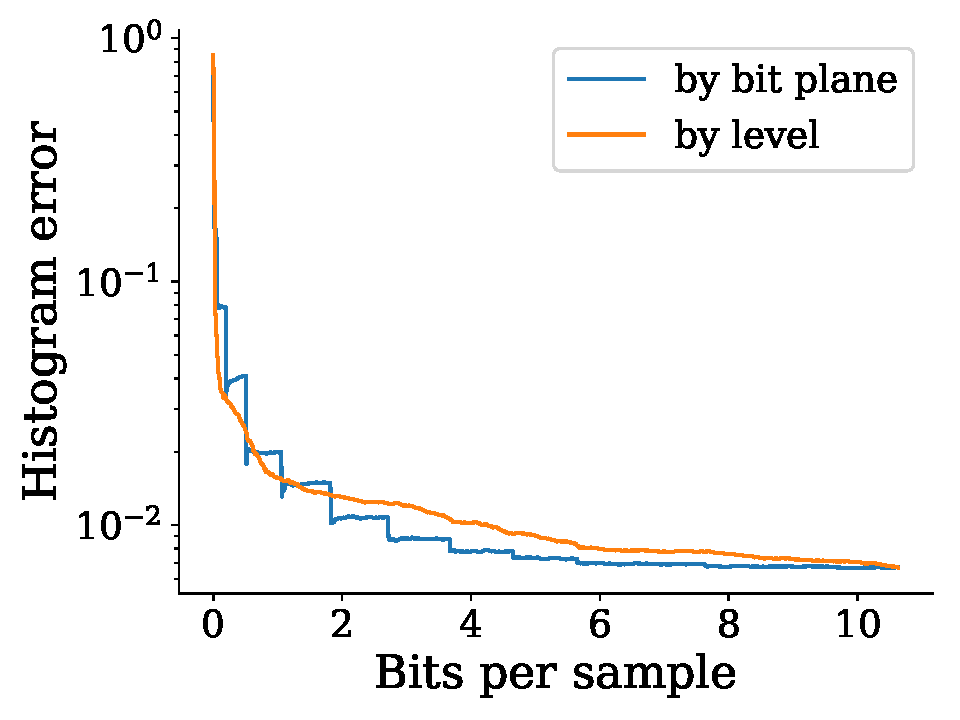
\includegraphics[width=0.48\linewidth]{histogram/histogram-explain-boiler}} \caption{Comparison
	of histogram error curves produced by $s_{bit}$ and $s_{lvl}$, for \emph{boiler}, with and without
	leading zero bits. The vertical axis is in log scale. The error for $s_{bit}$ reduces in a
	stair-step fashion, in which each step corresponds to a new bit plane streamed. $s_{bit}$ benefits
	significantly more from the removal of leading zero bits (from (a) to (b), the blue curve shifts
	more to the left).}
	\label{fig:histogram-explain}
\end{figure}

\begin{figure}[t]
	\centering
	\subcaptionbox{\emph{by level} ($s_{lvl}$)}{
	{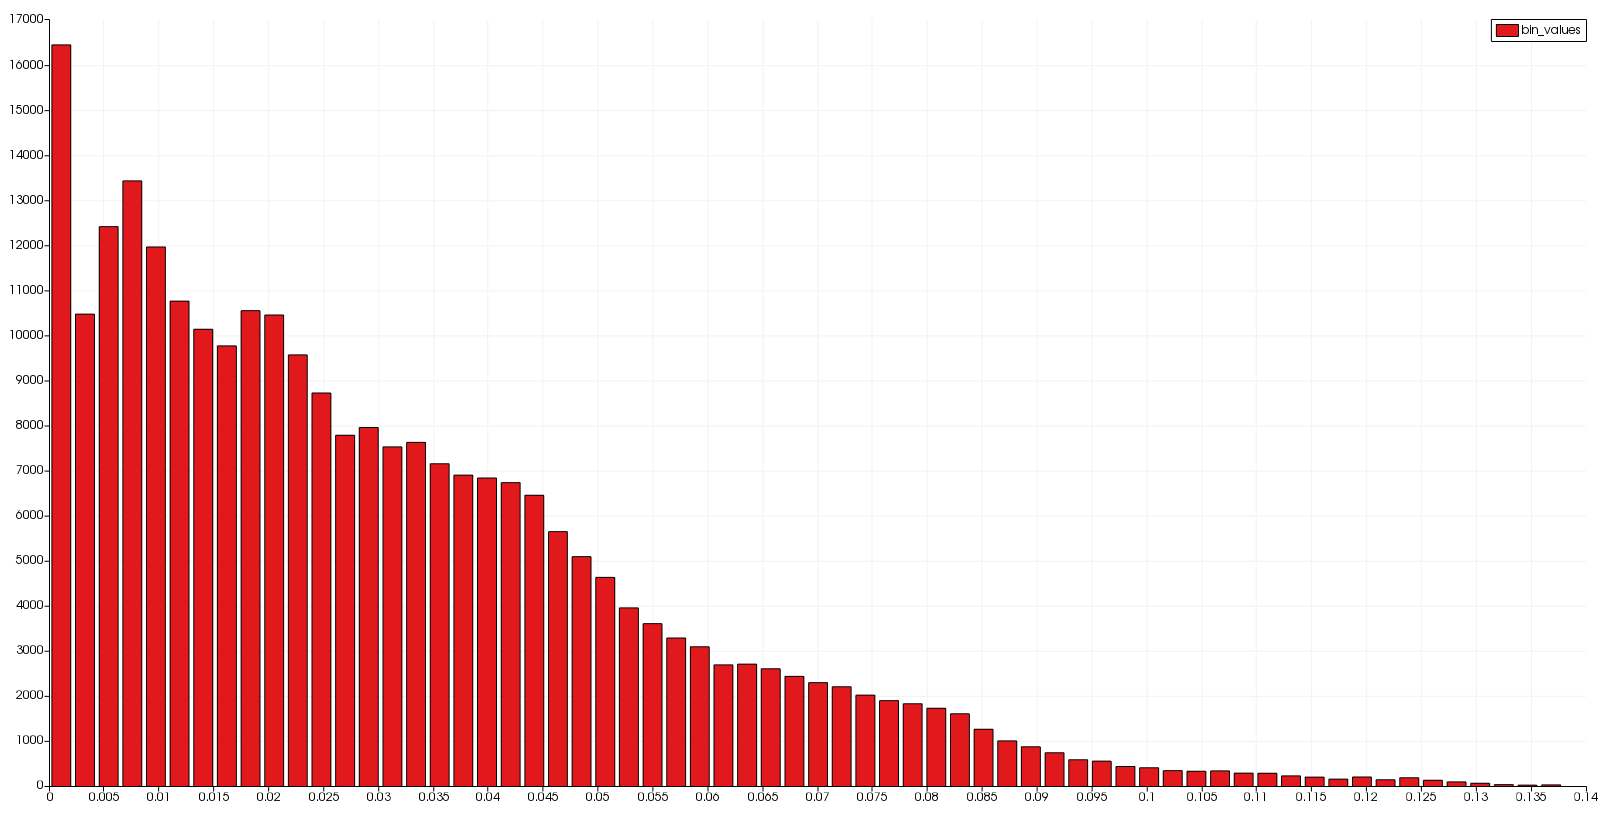
\includegraphics[width=0.31\linewidth]{histogram/histogram-boiler-level.png}}}
	\subcaptionbox{\emph{by bit plane} ($s_{bit}$)}{
	{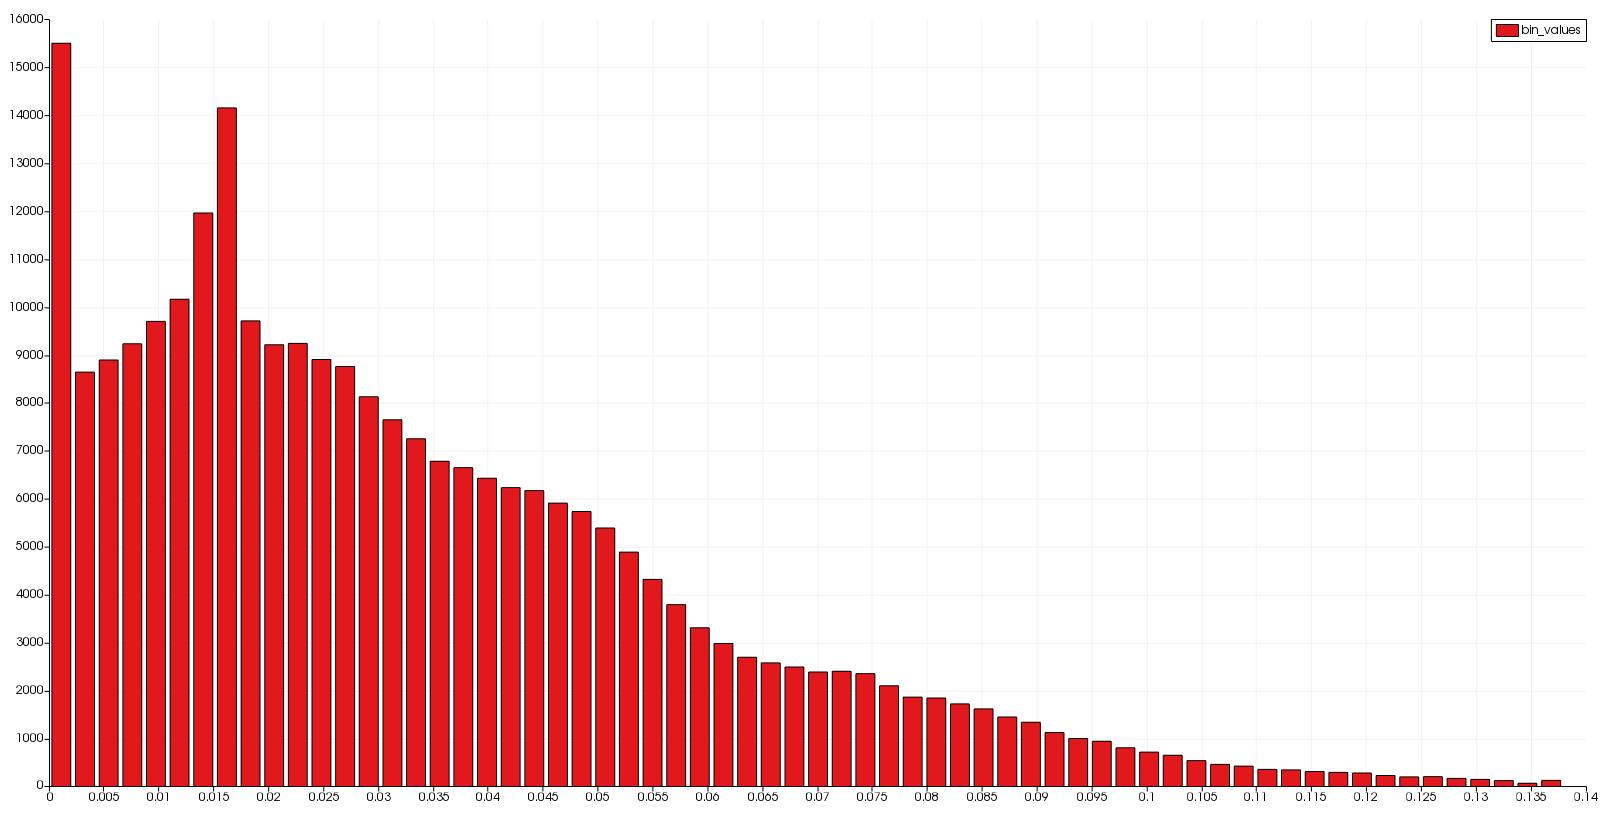
\includegraphics[width=0.31\linewidth]{histogram/histogram-boiler-bit-plane.png}}}
	\subcaptionbox{\emph{by magnitude} ($s_{mag}$)}{
	{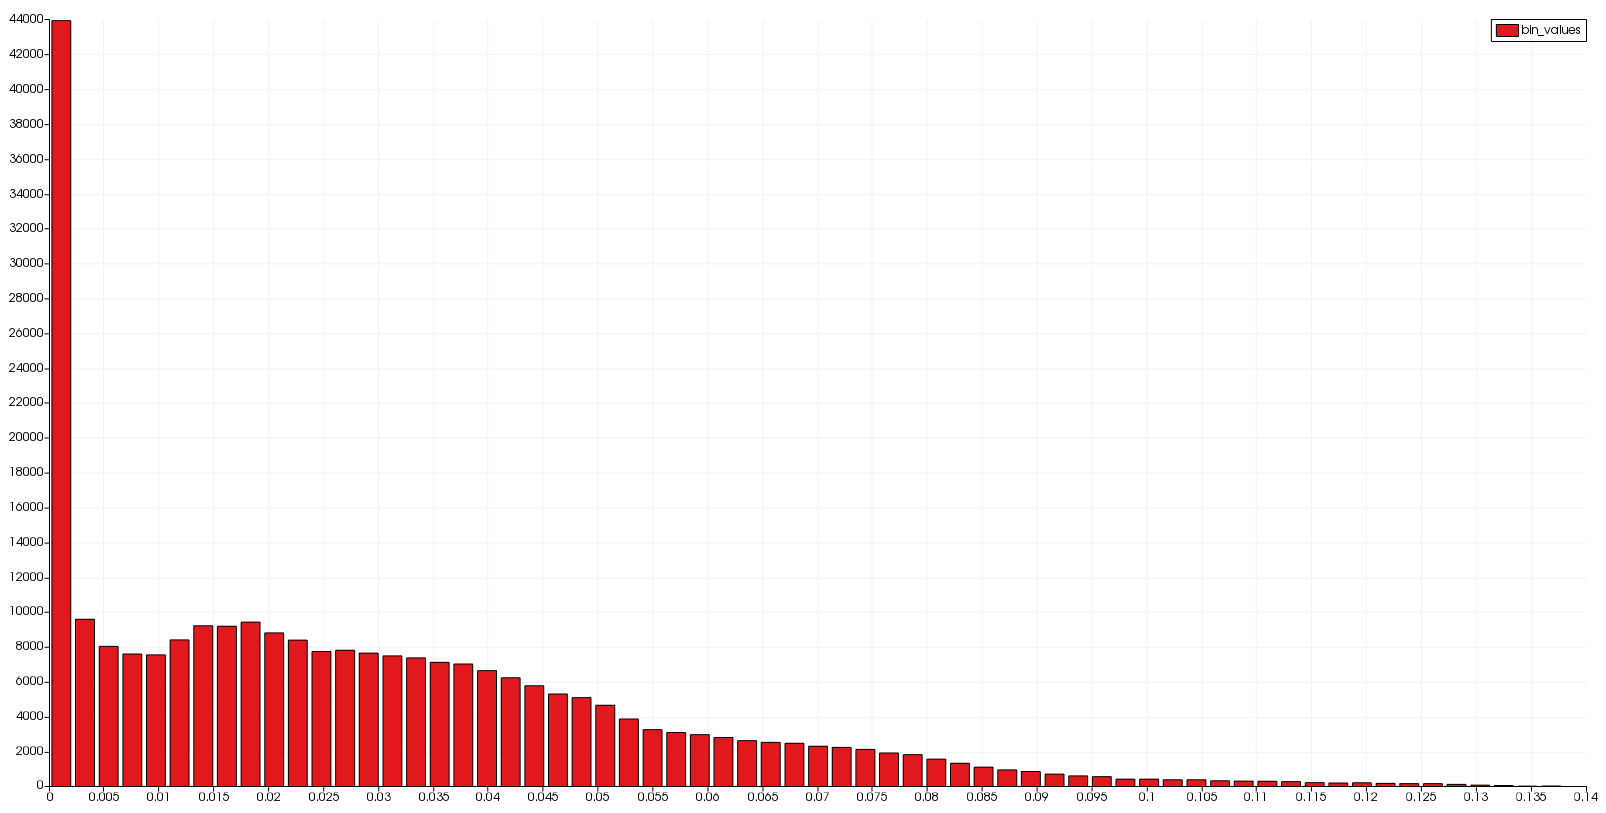
\includegraphics[width=0.31\linewidth]{histogram/histogram-boiler-magnitude.png}}}
	\subcaptionbox{\emph{by wavelet norm} ($s_{wav}$)}{
	{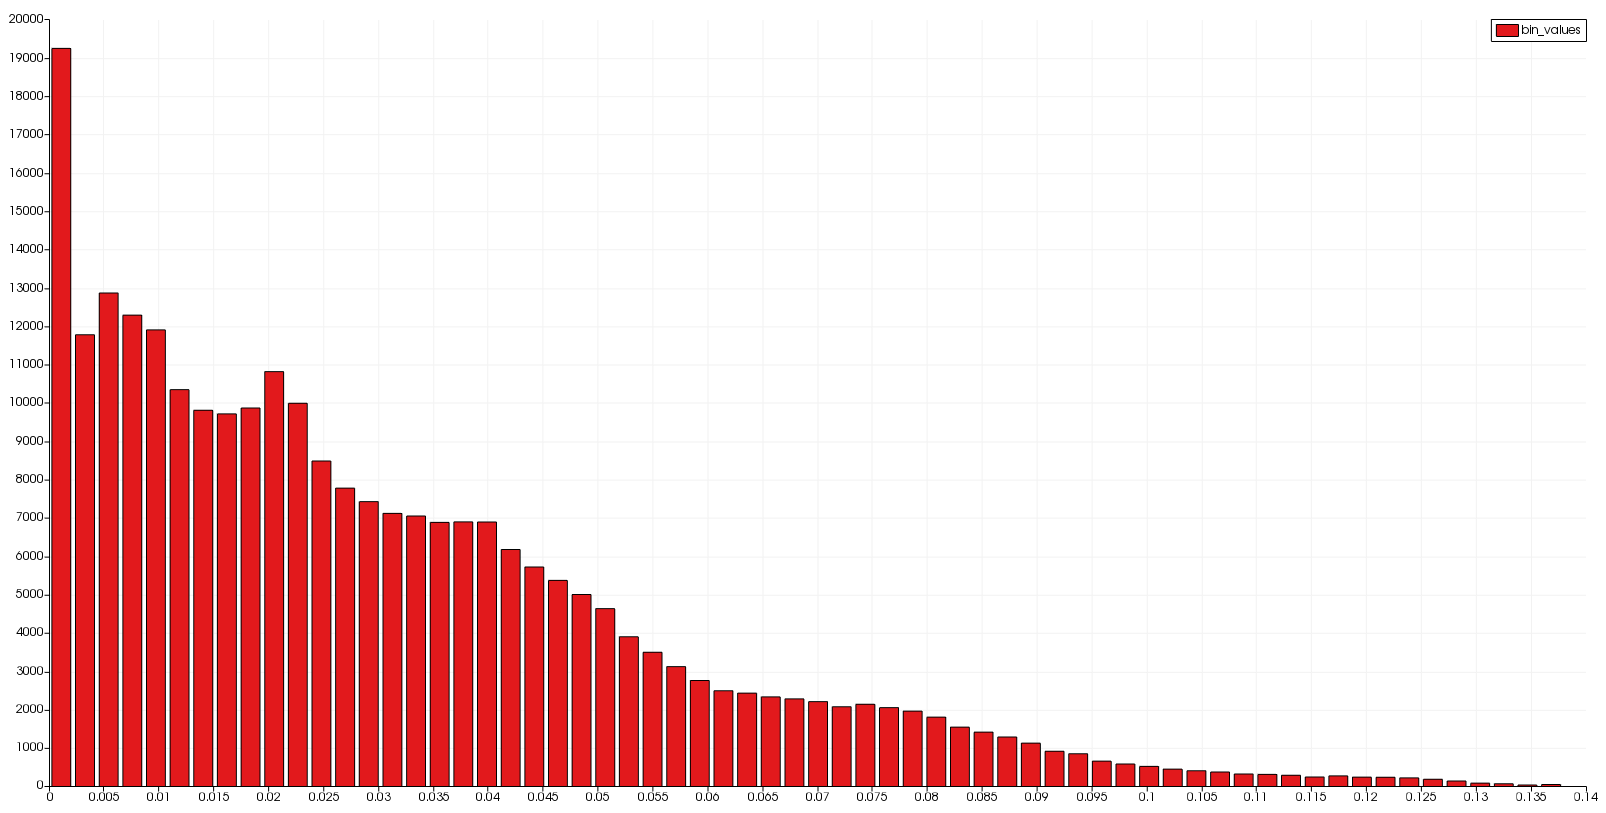
\includegraphics[width=0.31\linewidth]{histogram/histogram-boiler-wavelet-norm.png}}}
	\subcaptionbox{\emph{by signature} ($s_{hist-sig}$)}{
	{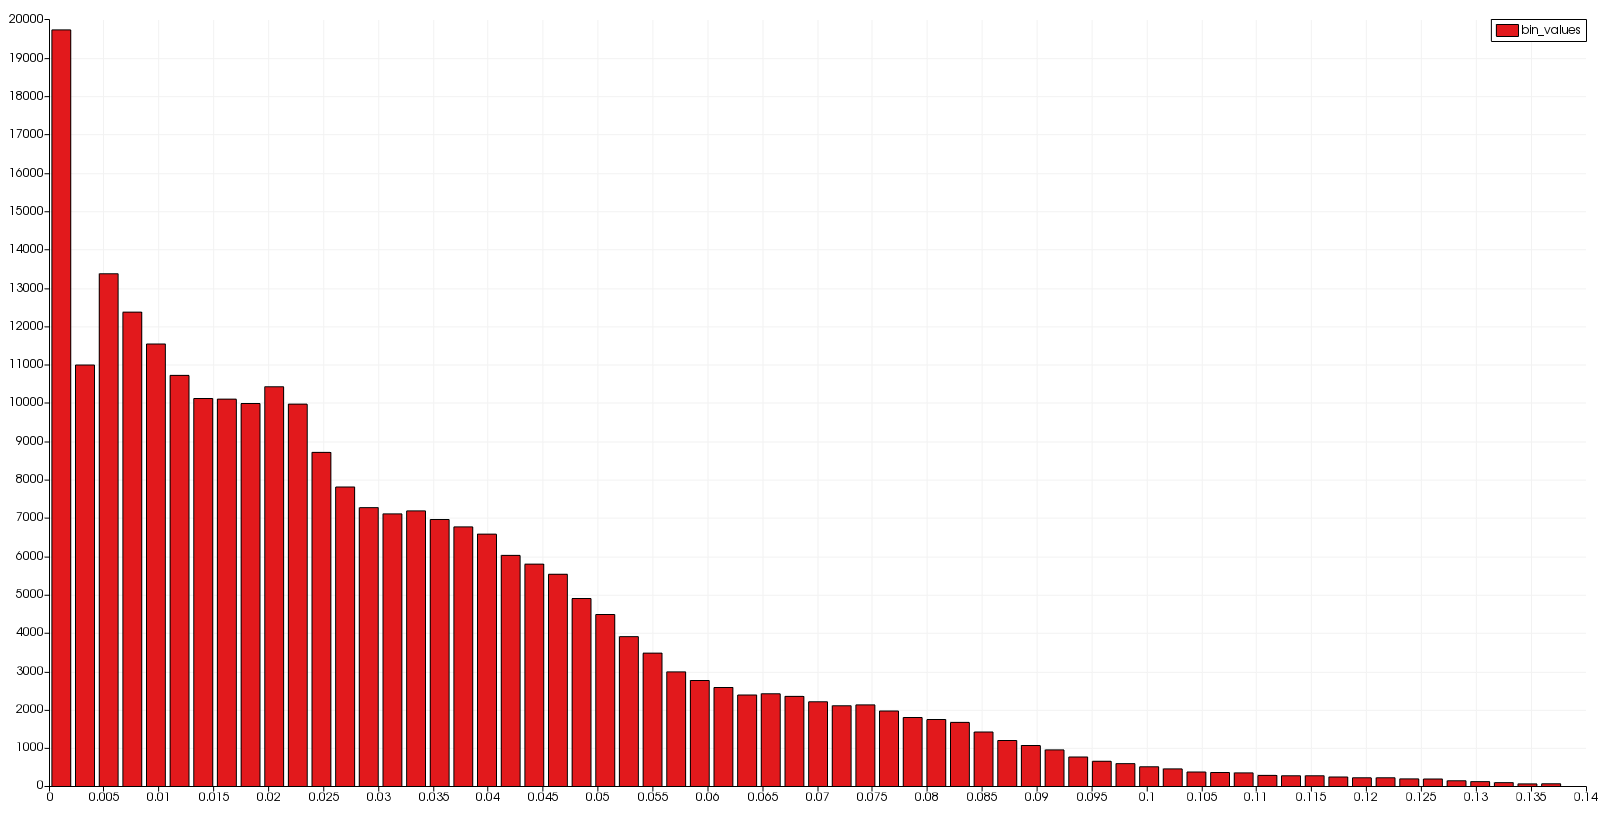
\includegraphics[width=0.31\linewidth]{histogram/histogram-boiler-signature.png}}}
	\subcaptionbox{\emph{reference}}{
	{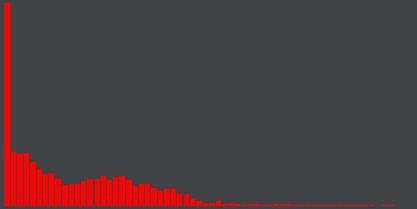
\includegraphics[width=0.31\linewidth]{histogram/histogram-boiler-groundtruth.png}}}
	\caption{Histograms of the \emph{boiler} data set, reconstructed at 0.08 bps. $s_{lvl}$,
	$s_{wav}$, and $s_{hist-sig}$ produce histograms share similar shape to the reference histogram,
	with most of the peaks and valleys preserved. In contrast, $s_{bit}$ produces a spurious peak not
	found in the reference. Finally, $s_{mag}$'s histogram has a widely skewed distribution where too
	many values fall into the first bin.}
	\label{fig:histograms-boiler}
\end{figure}

% \pavol{summarize subsection}
% In summary, we have evaluated six data sets, for each using different histogram streams, and
% compared results with respect to the histogram intersection error and the visual differences.
% Interestingly, the order of streams differs from all the other queries, where {\em by level} stream
% performed poorly, but for histograms it outperforms both {\em by magnitude} and {\em by bit plane}
% streams. The idea of signature works for histograms as well, and could be employed as a practical
% streaming format, where the sender would first send the signature to the receiver at small cost (few
% integer values). However, {\em by wavelet norm} stream has similar performance and does not require
% any extra data transfered (such as signature), and thus we conclude that from considered streams it
% has best properties.

% \pavol{The visualization of the subbands is missing, but I think it was quite interesting and maybe we
% should find a way to include it as it makes the discussion more interesting.}
